\chapter{Grammatical Sutta Finder}\label{chap:gramsutfinder}

This tool is designed for advanced learners who are familiar, or in the course of learning, with traditional Pāli grammar books.

In the three schools of Pāli grammar (namely Kaccāyana, Moggallāna, and Saddanīti), the main part of their textbooks is grammatical suttas. These suttas are terse formulas that explain grammatical points. The suttas themselves are sometimes, if not most of the time, unintelligible to the uninitiated. So, those who see the usefulness of the tool have to be familiar with these grammar books in some degree.

In this tool, all suttas taken from the grammar books and their main commentaries are listed. These books are Kaccāyanabyākara (Kacc or k) with Padarūpasiddhi (Rūpa or r), Moggallānabyākara (Mogg or m) with Payogasiddhi (Payo or p) and Niruttidīpanī (Niru or n), and Saddanīti Suttamālā (Sadd-Sut or s), totally 5,263 suttas in 6 books.\footnote{The majority of suttas in each school are repeated in their commentaries, slightly different sometimes. And some suttas are equivalent across schools. So, total distinct suttas are not so many (but still numeruous to remember them all).}

The window of Grammatical Sutta Finder is shown in Figure \ref{fig:gramsut-finder}. With {\faSix \symbol{"F0AE}} toggle button, you can turn on and off the book selectors.

\begin{figure}[!hbt]
\centering
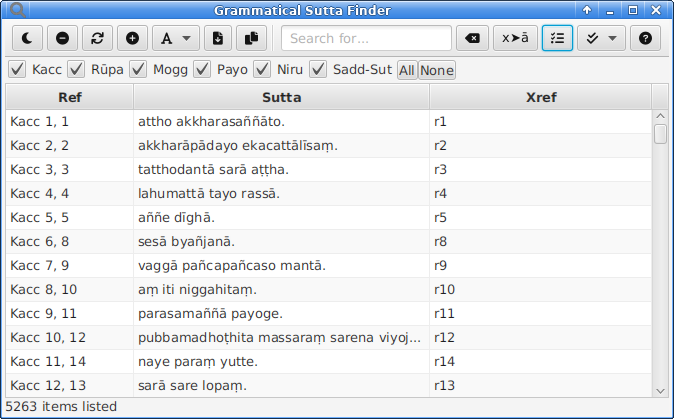
\includegraphics[width=0.9\linewidth]{images/gramsut-finder.png}\\
\caption{Window of Grammatical Sutta Finder}
\label{fig:gramsut-finder}
\end{figure}

In the result table, each item or sutta has its reference, its sutta body, and cross-references that link to related works. For example, in Kacc the related suttas of Rūpa will be given, and vice versa.\footnote{It is somewhat redundant here because the number of Rūpa sutta is already given in Kacc suttas. But in Rūpa cases, the table can be helpful.} In the school of Mogg, all three books are related together. For Sadd-Sut has no commentary here, its suttas are blank in this column. 

\begin{figure}[!hbt]
\centering
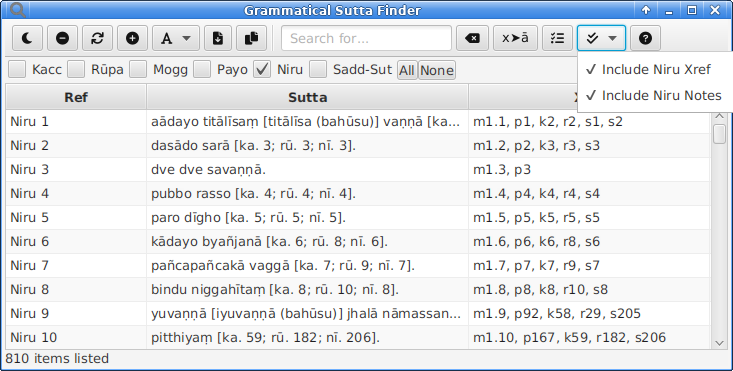
\includegraphics[width=0.9\linewidth]{images/gramsut-niru.png}\\
\caption{Suttas of Niruttidīpanī in full}
\label{fig:gramsut-niru}
\end{figure}

Niruttidīpanī by Leḍī Sayāḍo plays a significant role in providing additional cross-reference information, as shown in notes in each sutta of this book. To enable this, you have to select {\faSix \symbol{"F00C}} Include Niru Xref in {\faSix \symbol{"F560}} menu button. To enable the notes in Niru's suttas, you have to select likewise the nearby menu. Figure \ref{fig:gramsut-niru} shows suttas in this book in full options. Even though Sadd-Sut has no references to other books, it can be related to others in this way.

The search function, in this tool is versatile. It can search a string in the sutta body. It can also search in the cross-references with the short form. Figure \ref{fig:gramsut-search} illustrates an attempt to find related suttas of Sadd 1119. This can be done even if the option of Include Niru Xref is turned off. From this information, you can trace explanations in other schools.

\begin{figure}[!hbt]
\centering
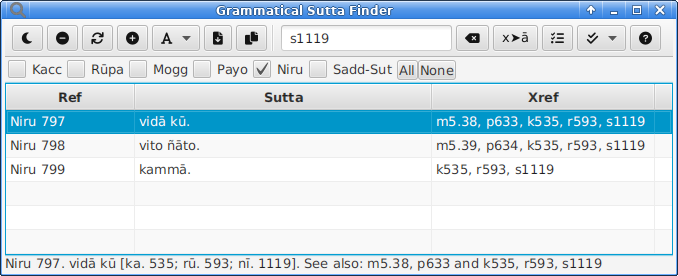
\includegraphics[width=0.9\linewidth]{images/gramsut-search.png}\\
\caption{Searching a reference}
\label{fig:gramsut-search}
\end{figure}

Moreover, you can just enter a book's initial uppercase in the search field to show only suttas of that book, i.e., K, R, M, P, N, and S. Figure \ref{fig:gramsut-search-book} shows only suttas from Padarūpasiddhi.\footnote{The full abbreviation (Rūpa) also works but more expensive.}

\begin{figure}[!hbt]
\centering
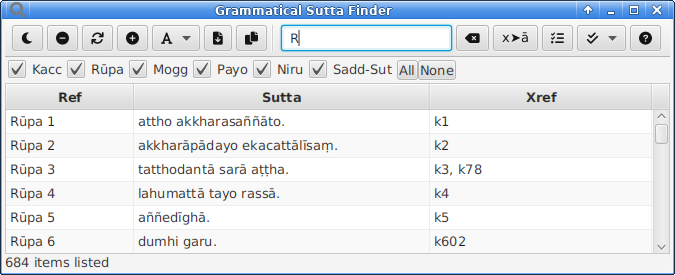
\includegraphics[width=0.9\linewidth]{images/gramsut-search-book.png}\\
\caption{Showing one book by searching its initial}
\label{fig:gramsut-search-book}
\end{figure}

